\subsection{RQ3: Target specification on a public common prediction support}\label{subsec:result-eval}
The CTRPv2 LCO target panel contains $106{,}696$ unique curve-summary rows shared by all $34$ stored predictors, including five naive baselines. We compare the $29$ non-naive models on these same observations and fixed predictions. FULL uses ordinary $R^2(y,p)$ and $\operatorname{corr}(y,p)$; ID uses $R^2(Qy,Qp)$ and $\operatorname{corr}(Qy,Qp)$, removing held-out cell-line offsets. Each compound--cell-line--fold key is unique in the source and included predictions. Baseline-normalized scores constitute a separate protocol.

By Theorem~\ref{eq:duality}, projecting onto the reference-resolved subspace $\operatorname{range}(Q)$ eliminates unresolved cell-line offsets ($U^\top Q=0$), reversing a median $4.56\%$ of foldwise $R^2$ pair orders and $2.83\%$ of Pearson orders (Table~\ref{tab:publictargets}; Fig.~\ref{fig:publictargets}). ElasticNet--MOLIR, KNNRegressor--MOLIR and Lasso--MOLIR reverse in all ten folds. Their median A-minus-MOLIR $R^2$ margins change from $+0.1305$ to $-0.1225$, $+0.1276$ to $-0.0948$, and $+0.1257$ to $-0.1307$, respectively. The mean $R^2$ leader changes from SingleDrugRandomForest to EnsembleMF. These persistent all-fold inversions confirm that ambient and quotient targets evaluate structurally distinct response components on identical predictions. The five-model companion panel has $210{,}741$ unique common rows and median reversal fractions $10.0\%/5.0\%$, with no persistent pair outcome; RandomForest leads under both targets.

\begin{table}[t]
\centering\small\setstretch{1.05}
\caption{Public LCO common-support target analysis. FULL uses ordinary raw-response $R^2$/Pearson; ID uses $Qy,Qp$. Percentages are medians over ten folds, and persistent outcomes require the same directed reversal in at least seven folds. These exploratory panels are separate from the historical baseline-normalized LDO protocol.}
\label{tab:publictargets}
\begin{tabularx}{\textwidth}{@{}L{0.18\textwidth}N{0.12\textwidth}N{0.08\textwidth}N{0.09\textwidth}X@{}}
\toprule
 & & \multicolumn{2}{c}{\PAIRTableHead{Median reversal}} & \\
\cmidrule(lr){3-4}
\PAIRTableHead{Panel} & \PAIRTableHead{Unique common rows} & \PAIRTableHead{$R^2$} & \PAIRTableHead{Pearson} & \PAIRTableHead{Persistent outcomes and mean $R^2$ leader}\\\midrule
29 non-naive models; 5 baselines bound & $106{,}696$ & $4.56\%$ & $2.83\%$ & Three $R^2$ pairs, each $10/10$ folds; SingleDrugRandomForest $\to$ EnsembleMF.\\
Five classical/literature models; common baseline bound & $210{,}741$ & $10.0\%$ & $5.0\%$ & Zero persistent pairs; RandomForest under both targets.\\\bottomrule
\end{tabularx}
\end{table}

\begin{figure}[t]
\centering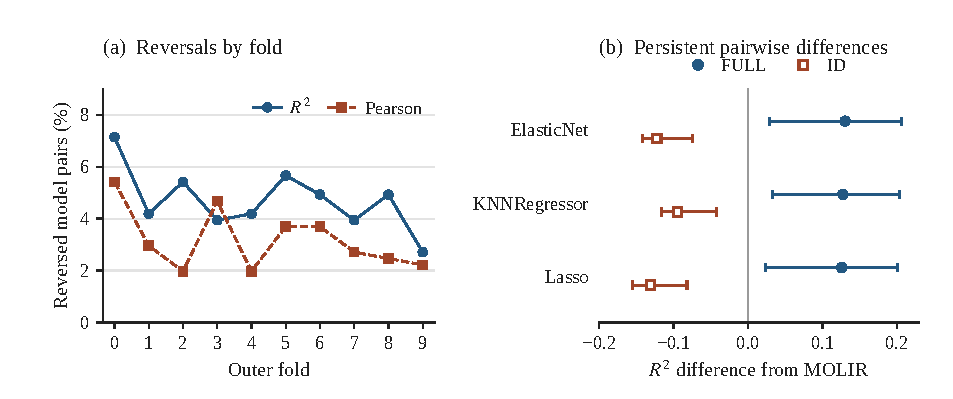
\includegraphics[width=\textwidth]{figures/public_target_comparison.pdf}
\caption{\textbf{Scoring-target sensitivity on fixed public LCO predictions.} \textbf{(a)} Foldwise reversal fractions on the $29$-model unique common support under ordinary raw-response versus quotient targets. \textbf{(b)} Model-minus-MOLIR $R^2$ differences under FULL and ID. Points mark ten-fold medians and horizontal lines span the observed minimum--maximum differences. Each comparison reverses direction in all ten folds; all three involve MOLIR. The two targets describe different prediction components.}
\label{fig:publictargets}
\end{figure}

A separate sparse least-squares residualization reconstructs all $400$ stored model--fold records in the two panels, with maximum absolute numerical discrepancy $2.92\times10^{-11}$ across the checked scalar fields. Classical within-cell centering gives the same quotient action on these connected supports. The scientific choice is the response component required by the application, while the reference geometry makes that choice explicit.

Complementary baseline-normalized panels delimit persistence across protocols. The seven-model CTRPv2 LDO study has median reversals $50.0\%/35.7\%$ and five persistent pair--metric outcomes on model-specific supports, one recurring under symmetric-HPO retraining. The six-model common-support GDSC2 and GDSC1 panels have median reversals $30.0\%/30.0\%$ and $37.0\%/33.0\%$, with zero persistent outcomes; the prespecified GDSC2 confirmation is unmet. Their exact projectors and within-drug centering agree on all $300$ ranking checks (Sections~S4 and S17). The ENCODE fixed-prediction study similarly yields M2--M3--M1 under compound-only loss and M3--M2--M1 under unitwise-supported loss (Section~S3.3).

\subsection{RQ4: Observation weights change numerical model comparisons}\label{subsec:result-measure}
The normalized-score path in the frozen DrEval LCO release joins baseline predictions by drug, cell line and fold without requiring a unique right-hand key. Over $340$ model--fold records it expands $7{,}160{,}483$ finite native rows to $7{,}461{,}981$ joined rows. Reconstructed normalized $R^2$ and Pearson match the archived outputs to $3.91\times10^{-14}$ and $6.11\times10^{-16}$. This reconstruction isolates the measure-distortion mechanism within the bound public snapshot while maintaining strict provenance separation from external production runs.

The $29$-model matched panel retains $112{,}066$ original curve-summary records over $109{,}298$ keys. Repeated keys enter only when truth and multiplicity match the official split and one numerical baseline value exists. Its $106{,}696$ singleton keys are exactly the RQ3 support. The $2{,}602$ duplicated lookup keys produce $117{,}934$ rows under the unchecked join. Requiring one baseline value per key preserves every original record once, satisfying Eq.~\eqref{eq:measurepreserve}, without inventing pairings between ambiguous occurrences.

\begin{table}[t]
\centering\small\setstretch{1.05}
\caption{Consequences of duplicate baseline lookup on the fixed $29$-model panel. Each fold has $\binom{29}{2}=406$ pairs. Top-three changes count folds or the single mean-score panel, rather than pairwise comparisons.}
\label{tab:measureimpact}
\begin{tabularx}{\textwidth}{@{}XN{0.16\textwidth}N{0.17\textwidth}N{0.23\textwidth}@{}}
\toprule
\PAIRTableHead{Comparison} & \PAIRTableHead{Strict pair reversals} & \PAIRTableHead{First-place changes} & \PAIRTableHead{Top-three membership changes}\\\midrule
Fold normalized $R^2$ & $24/4{,}060$ & $0/10$ folds & $3/10$ folds\\
Fold normalized Pearson & $37/4{,}060$ & $0/10$ folds & $4/10$ folds\\
Ten-fold mean normalized $R^2$ & $5/406$ & $0$ & $1$\\
Ten-fold mean normalized Pearson & $0/406$ & $0$ & $0$\\\bottomrule
\end{tabularx}
\end{table}

The altered weights reverse $61/8{,}120$ fold pair--metric orders ($0.75\%$) and $5/812$ mean pair--metric orders ($0.62\%$; Table~\ref{tab:measureimpact}). In mean normalized $R^2$, EnsembleMF and RandomForestAEMolGNet exchange third and fourth place. The two mean-score leaders remain unchanged. Thus pair-order changes, shortlist membership and first-place selection are different consequences of the same mechanism.

All $66$ repair witnesses are verified from frozen sufficient statistics. Exact minimum key counts range from $1$ to $71$ (median $2$) for the $24$ fold normalized-$R^2$ reversals and from $5$ to $56$ (median $8$) for the five mean reversals. Pearson minimality is closed in $34/37$ cases; three retain lower--upper intervals. For the EnsembleMF--RandomForestAEMolGNet shortlist comparison, the A-minus-B mean margin changes from $+0.000765$ to $-0.001172$. Six keys suffice to reverse its unchecked order, and every smaller set is excluded under that repair definition. Treating the $15$ affected cell-line lookup groups as the action unit instead gives minimum counts of $1$--$2$ groups per fold and $1$--$4$ per mean reversal (Section~S18). The intervention unit is therefore part of the certificate.

\begin{figure}[t]
\centering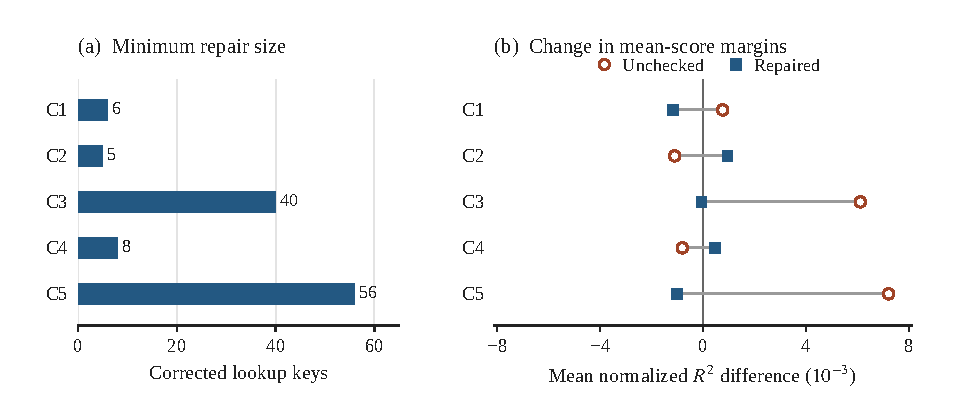
\includegraphics[width=\textwidth]{figures/repair_and_materiality.pdf}
\caption{\textbf{Localizing the five mean normalized-$R^2$ reversals.} \textbf{(a)} Minimum numbers of duplicate lookup keys to correct. \textbf{(b)} Pairwise mean-score differences before and after cardinality-preserving repair. Case identifiers map to model pairs in Supplementary Section~S18. None of the five cases has an absolute margin of at least $0.005$ on both sides of the repair.}
\label{fig:repairimpact}
\end{figure}

The mean effects are sensitive to aggregation. Four of the five mean pair reversals occur without a within-fold sign change for that pair: changes in foldwise margins suffice to reverse their average. Deleting one fold at a time retains each mean reversal in only $1$--$4$ of ten deletions, and none has margins of at least $0.005$ on both sides. Together, these sensitivity diagnostics quantify the practical materiality of join-induced weight distortions across fold-level and aggregate leaderboards. Additional baseline-coverage checks on GDSC2, GDSC1, CCLE and CTRPv1 produce no reversals in the five-model primary panels; a secondary eight-model GDSC2 panel has one foldwise normalized-$R^2$ change and no changed mean leader (Section~S18.5).

\FloatBarrier
\subsection{RQ5: Decision sufficiency and sequential evidence disclosure}\label{subsec:result-certificates}
The AMLB snapshot~\cite{gijsbers2024amlb} contains a genuine record gap: the four-hour \texttt{autosklearn} run on \texttt{socmob} lacks fold $9$. Reconstructing the upstream cleaning and aggregation reproduces $29{,}829$ entries. Allowing the absent score to vary over $x=-\mathrm{RMSE}\le0$, with all other scores fixed, yields $26$ regression and $22$ all-task boundary/interval states, including ties. AutoGluon(B) remains the unique winner and the same top-three members are retained throughout both domains.

The analytic interval certificate gives positive conservative winner gaps of $1.151515$ and $1.576923$ mean-rank units, and top-three separation gaps of $0.348485$ and $0.245192$ (Eq.~\eqref{eq:intervalcert}). Complete regime enumeration tightens the minimum winner gaps to $1.181818$ and $1.586538$. The graph retains $12+10=22$ winner--challenger certificates with the absent job, admissible domain and endpoint witness (Section~S19).

Whole-task deletion supplies a separate population stress test. All eight budget/metric panels retain their winner after any single task deletion. The one-hour regression and AUC panels permit $9$ and $4$ single-task top-three membership changes, plus one regression boundary tie. Minimum strict winner overturns require $6$--$39$ complete task deletions across the eight panels. Integer witnesses verify all $94$ challenger comparisons; $221$ exhaustive small-panel checks agree. The full panel table is retained in Section~S19.

TabArena~\cite{erickson2025tabarena} permits verification at the prediction-row level. Default Mitra\_GPU and LightGBM configurations share $654$ evaluation units across $33$ OpenML tasks: $20$ binary, six multiclass and seven regression. Their $1{,}308$ prediction records contain $1{,}251{,}480$ rows and $155{,}583$ distinct task--row identities. Test identities, order and labels match canonical references; validation labels match their corresponding training splits.

A separate metric implementation reproduces all $1{,}308$ cached scores, while execution of the fixed test-ensemble aggregation preserves the predictions. Native versus replayed scores produce zero order or tie-status changes over $654$ unit comparisons and $33$ task means, retaining the same $31$--$2$ task-win split. The smallest observed ratio of pair margin to combined native-to-reconstruction score deviation is $32.0$. These results cover the two common defaults.

Observed agreement and production identity are distinct qualifications. Of $1{,}308$ native score fields, $43$ in $31$ evaluation units fall outside a conditional single-Float32-rounding model: $37$ log-loss values on \texttt{anneal} and six AUC values. Historical internal predictions, clipping order and library versions remain unresolved. Four pairwise rounding enclosures include zero despite unchanged observed orders; all $33$ task-mean enclosures have a strict direction under that model (Section~S20).

\paragraph{How much evidence suffices for a fixed-pool decision?}
Sequential disclosure asks when the same fixed comparison becomes decidable. The 26 eligible classification tasks contain $43{,}007$ canonical labels: $20$ binary AUC tasks and six multiclass log-loss tasks. We use each task's first common metadata-ordered split and the same Mitra\_GPU/LightGBM predictions. Archived labels are masked and disclosed under the fixed metric and completion domain.

Under the same strict completion rule, random disclosure needs $95.76\%$ of each pool on average, compared with $92.15\%$ for predictive entropy, $77.97\%$ for interval width, $68.67\%$ for fixed expected gain and $65.44\%$ for adaptive expected gain (Fig.~\ref{fig:disclosure}). The adaptive rule requires fewer labels than the mean random path on all 26 fixed pools. The mean absolute reduction is $30.32$ percentage points; the mean of the per-task relative reductions is $32.09\%$. These two summaries use different denominators. All $1{,}404$ paths terminate at a correct certificate for the fully disclosed pool.

\begin{figure}[t]
\centering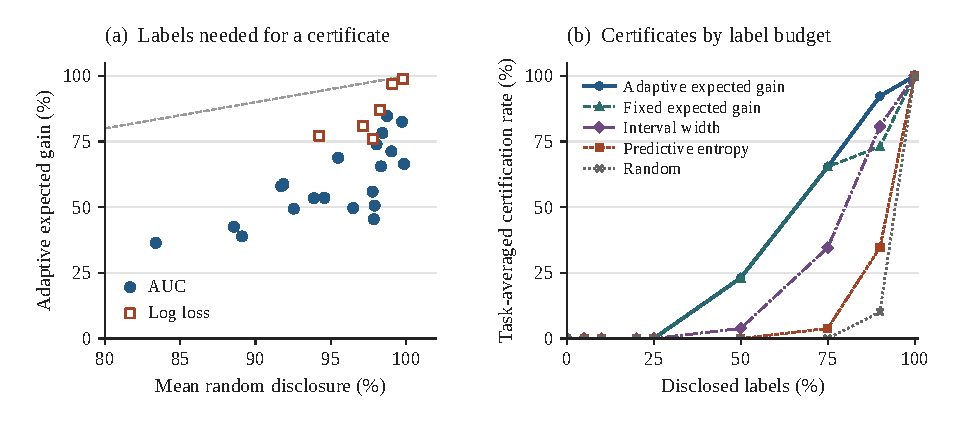
\includegraphics[width=\textwidth]{figures/sequential_disclosure.pdf}
\caption{\textbf{Decision-certified disclosure on frozen prediction pools.} \textbf{(a)} Label fractions required by adaptive expected gain and mean random disclosure, with one point per task. \textbf{(b)} Task-averaged certification rates at the recorded label budgets. Counts concern existing archived labels. Fixed predictions, canonical row identities, a shared completion domain and the same stopping rule are held constant across policies.}
\label{fig:disclosure}
\end{figure}

The pooled result covers distinct regimes: adaptive disclosure averages $59.21\%$ for AUC and $86.20\%$ for log loss. It is also prior-sensitive. Post hoc replacement of the pooled probability prior gives $63.81\%$ with Mitra probabilities, $73.06\%$ with LightGBM probabilities and $77.97\%$ with uniform class probabilities. Mitra wins 23 of these 26 complete-pool comparisons; its prior improves 17 acquisition paths, leaves two unchanged and worsens seven. These results describe this model collection and do not select a new prior using the test outcomes.

Two separate numerical controls support the stopping certificates. Generic same-domain LPs agree on 104 endpoints before and at adaptive stopping, with maximum difference $5.68\times10^{-14}$. A separate exact-arithmetic implementation imports neither the production policy nor its bound and stopping routines; it reproduces all $1{,}404$ paths and verifies $2{,}808$ stopping-prefix checks. Re-execution of the scoped VMA query-function adapter reproduces all $600$ frozen control paths byte for byte. On six log-loss tasks that function requires $97.72\%$ of labels versus $97.75\%$ for its matched random sampler under the same strict certificate. The six-task hindsight minimum averages $78.09\%$; it uses all answers. Section~S23 gives the task-level results and precise query-function scope, including its distinction from the full VMA/LURE procedure.

Collectively, these results demonstrate that strict decision certificates emerge substantially before full pool disclosure, while decoupling heuristic acquisition policies from the policy-agnostic algebraic verifier and its source-bound budget record.

The joint representation and matched classical control are evaluated next.
